\documentclass[10pt]{article}
\usepackage[a4paper,margin=1in]{geometry}
\usepackage[T1]{fontenc}
\usepackage{mathptmx}
\usepackage{microtype}
\usepackage{graphicx,booktabs,array,xcolor,amsmath}
\usepackage{tikz}
\usetikzlibrary{arrows.meta,positioning,shapes.geometric}
\usepackage[colorlinks=true,linkcolor=blue!50!black,citecolor=blue!50!black,urlcolor=blue!50!black]{hyperref}
\usepackage{caption}
\captionsetup{font=small,labelfont=bf}
\setlength{\parindent}{0pt}\setlength{\parskip}{.55em}
\newcommand{\sig}{\textsc{SigMap}}
\newcommand{\ours}{\textsc{Ours}}
\newcommand{\ci}[2]{{\scriptsize[#1,\,#2]}}
\newcommand{\ind}[1]{\mathbf{1}\!\left[#1\right]}

\title{AST-Compressed Code Graphs for Gemma~4 Agents:\\ What a Small Local Model Gains from a Budgeted Repository Map}
\author{Muhammad Maroof\\ \small Independent researcher, Karachi, Pakistan \;\;\texttt{maroofiums@gmail.com}\\
\small Code and data: \url{https://github.com/maroofiums/astgraph-gemma}}
\date{Gemma 4 Developer Agent Paper Track}

\begin{document}
\maketitle

\begin{abstract}
\noindent Running a coding agent on a single consumer GPU means the repository cannot be pasted into the prompt, and a small model gets lost when it is. We build a repository map from tree-sitter ASTs (signatures, line ranges, optionally call edges and control-flow counts), rank symbols against the issue text, and fill a fixed token budget by score per token. We test it with Gemma~4 E4B (4-bit, one T4) on SWE-bench Lite issue localization, 150 test instances, with the ranker chosen on a separate dev split without any LLM calls. At a 2k-token budget a plain signature map reaches 0.527 file Acc@1 against 0.380 for function-snippet RAG and 0.280 for raw top-$k$ files, and doubles BM25 file ranking (0.267). Our richer variant, which adds call edges and control-flow counts, did \emph{not} help: it is 0.04 lower on file accuracy (not significant) and 0.09 lower on function accuracy ($p_{\text{Holm}}=0.002$). At function level, snippet RAG matches the signature map, and a two-stage prompt (map first, then candidate files) lifts function accuracy over the full variant (0.042 to 0.229 on the ablation subset) but not significantly over the plain signature map (0.188; difference $+0.042$, $p=0.54$). Memory measurements show that for this model the KV cache is a small part of what a long prompt costs; logits and activations dominate, and chunked prefill with last-token logits is what lets an 8k prompt be prefilled on a T4 (measured for prefill only). We also report the failure analysis, the negative results, and how the index can be used either as a prompt layer or as a set of tools.
\end{abstract}

\section{Introduction}
Most agent work on repository-level tasks assumes a large hosted model. If the model has to run locally, for privacy or cost, two problems show up together. The prompt budget is small, and the model is easy to distract. Pasting the files that a keyword search ranks highest spends the budget on method bodies the model does not need yet, and a model of Gemma~4 E4B's size (about four billion effective parameters) has little slack to ignore irrelevant text.

Repository maps are the usual answer. Aider's map lists files with the signatures of their most referenced symbols \cite{aider}; RepoGraph and CodexGraph go further and put a graph database behind the agent \cite{repograph,codexgraph}. What is less clear is which parts of such a representation matter for a small model, how the ranking interacts with the budget, and what the memory side looks like on 15\,GB of VRAM. This paper is a measured answer to those three questions, on one model and one task.

\paragraph{Task.} Given an issue and a repository checkout, name up to three files and one function where the fix belongs. Formally, for an issue text $q$ and a repository with file set $\mathcal F$, the model returns an ordered list $\hat F=(\hat f_1,\hat f_2,\hat f_3)\subseteq\mathcal F$ and one symbol $\hat s$; the reference patch defines the gold files $F^\star\subseteq\mathcal F$ and the set $L^\star$ of touched lines. This is the localization step of systems like Agentless \cite{agentless}; we do not generate patches.

\paragraph{Contributions.}
\begin{itemize}\itemsep0pt
\item An open implementation (\texttt{astgraph}) that builds a budgeted map from tree-sitter, with four rankers and a guarantee that the rendered text fits the budget.
\item A benchmark protocol with a dev split used only to pick the ranker (no LLM), a disjoint test split, bootstrap intervals and Holm-corrected paired tests.
\item Results that are partly negative: signatures carry the gain; call edges and control-flow counts, as we serialize them, do not.
\item A memory analysis of Gemma~4 E4B on a T4 that separates weights, KV cache and logits, and shows where the budget actually goes.
\end{itemize}

\section{Method}\label{sec:method}
\begin{figure}[t]\centering
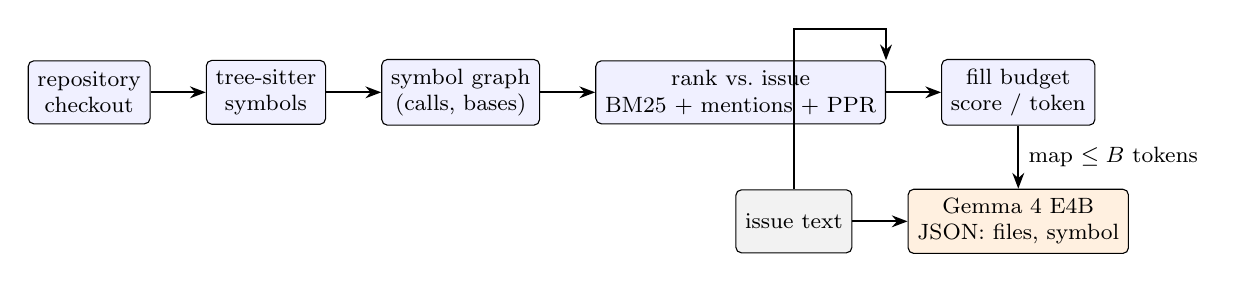
\begin{tikzpicture}[node distance=7mm, every node/.style={font=\footnotesize}, box/.style={draw,rounded corners=2pt,minimum height=8mm,align=center,fill=blue!6}, arr/.style={-{Stealth[length=2mm]},thick}]
\node[box] (repo) {repository\\checkout};
\node[box,right=of repo] (parse) {tree-sitter\\symbols};
\node[box,right=of parse] (graph) {symbol graph\\(calls, bases)};
\node[box,right=of graph] (rank) {rank vs.\ issue\\BM25 + mentions + PPR};
\node[box,right=of rank] (fill) {fill budget\\score / token};
\node[box,below=8mm of fill,fill=orange!12] (llm) {Gemma 4 E4B\\JSON: files, symbol};
\node[box,left=of llm,fill=gray!10] (issue) {issue text};
\draw[arr] (repo)--(parse); \draw[arr] (parse)--(graph); \draw[arr] (graph)--(rank); \draw[arr] (rank)--(fill);
\draw[arr] (fill)--node[right]{map $\le B$ tokens}(llm); \draw[arr] (issue)--(llm);
\draw[arr] (issue.north) |- ([yshift=4mm]rank.north east) -- (rank.north east);
\end{tikzpicture}
\caption{Pipeline. The map is rebuilt per issue from a cached parse; only the ranking and the fill step depend on the issue.}\label{fig:pipe}
\end{figure}

\paragraph{Symbols and graph.} For every \texttt{.py} file we parse with tree-sitter \cite{ts} and record, for each class, method and function, its qualified name, one-line signature (with annotations), line range, base classes, the names it calls, and counts of \texttt{if/for/while/try/with/match} nodes. Calls are resolved by name only, so an edge $a\to b$ means ``$a$ calls something called $b$'', weighted by $1/\#\text{candidates}$. Writing $V$ for the set of symbols, $\mathrm{callees}(a)$ for the names called inside $a$, and $C(n)=\{v\in V:\mathrm{name}(v)=n\}$ for the candidates of a name $n$, the edge weights are
\begin{equation}\label{eq:w}
w(a\to v)=\sum_{n\in\mathrm{callees}(a)}\frac{\ind{v\in C(n)}}{|C(n)|},
\end{equation}
so every call name spreads a total weight of at most one over its candidates. This is crude; there is no type inference. Files are keyed by SHA-1, so a re-index after a commit parses only changed files.

\paragraph{Ranking.} Each symbol $v$ becomes a small document $d_v$ (identifier words from its qualified name, its file path, and its callees). We score documents against the issue $q$ with BM25 \cite{bm25},
\begin{align}
\mathrm{bm25}(q,d)&=\sum_{t\in q}\mathrm{idf}(t)\,\frac{f_{t,d}\,(k_1+1)}{f_{t,d}+k_1\bigl(1-b+b\,|d|/\overline{|d|}\bigr)},\label{eq:bm25}\\
\mathrm{idf}(t)&=\ln\!\Bigl(1+\frac{|V|-\mathrm{df}_t+\tfrac12}{\mathrm{df}_t+\tfrac12}\Bigr),\notag
\end{align}
where $f_{t,d}$ counts term $t$ in $d$, $\mathrm{df}_t$ is the number of documents containing $t$, and $k_1,b$ are the usual BM25 constants. We compare four rankers. \textbf{bm25} uses $s_{\mathrm{bm25}}(v)=\mathrm{bm25}(q,d_v)$. \textbf{bm25m} adds a boost when the issue mentions the file path (including paths in tracebacks) or the symbol name (backticked, \texttt{snake\_case} or \texttt{CamelCase}):
\begin{equation}\label{eq:bm25m}
s_{\mathrm m}(v)=\mathrm{bm25}(q,d_v)+\delta_{\mathrm{path}}\,\ind{\mathrm{path}(v)\ \text{mentioned}}+\delta_{\mathrm{name}}\,\ind{\mathrm{name}(v)\ \text{mentioned}}.
\end{equation}
\textbf{ppr} is personalised PageRank \cite{pagerank} on the undirected graph with weights $\tilde w(u,v)=w(u\to v)+w(v\to u)$, seeded with the normalised BM25 scores $p_v=\mathrm{bm25}(q,d_v)/\sum_{u}\mathrm{bm25}(q,d_u)$:
\begin{equation}\label{eq:ppr}
r=\alpha\,P^{\top}r+(1-\alpha)\,p,\qquad P_{uv}=\frac{\tilde w(u,v)}{\sum_{x}\tilde w(u,x)},\qquad \alpha=0.5.
\end{equation}
\textbf{hybrid} mixes the two, both max-normalised:
\begin{equation}\label{eq:hybrid}
s(v)=0.7\,\bar s_{\mathrm m}(v)+0.3\,\bar r(v),\qquad \bar x(v)=\frac{x(v)}{\max_{u}x(u)}.
\end{equation}

\paragraph{Budgeted rendering.} Candidates are the top 3000 symbols $V_{3000}$ by $s$. Each has a cost $\tau$: the length of its rendered line in tokens, plus the file path the first time its file appears. For a symbol $v$ in file $\pi(v)$, given the set $S$ already chosen,
\begin{equation}\label{eq:cost}
\tau(v\mid S)=\ell(v)+\ell\bigl(\pi(v)\bigr)\,\ind{\pi(v)\notin\pi(S)},
\end{equation}
where $\ell(\cdot)$ is a token length. The map is a greedy solution of the knapsack-style problem
\begin{equation}\label{eq:knap}
\max_{S\subseteq V_{3000}}\ \sum_{v\in S}s(v)\qquad\text{s.t.}\qquad \sum_{v\in S}\tau\bigl(v\mid S_{<v}\bigr)\le B,
\end{equation}
where $S_{<v}$ are the symbols added before $v$: we take symbols in decreasing order of score per token, $s(v)/\tau(v)$, and keep each one while it fits. This is not optimal in general. Files are listed by their best score, $s(f)=\max_{v\in f}s(v)$. The final text is re-counted and trimmed if the greedy estimate was off, so that $|\mathrm{tok}(\mathrm{render}(S))|\le B$ always holds and the budget is a hard limit. A row looks like \texttt{m def parse\_date(self, s) -> str L41-58}; the optional suffixes are \texttt{>callee1,callee2} and \texttt{\#if2 for1}.

\paragraph{Prompt.} The system prompt asks for JSON only: up to three files and one qualified symbol. The map goes first, the issue (truncated to 1024 tokens for every method) after it, and decoding is greedy with at most 200 new tokens. Predictions are parsed leniently; a symbol is cleaned of \texttt{def}, file prefixes and argument lists.

\section{Experimental setup}
\paragraph{Model and hardware.} \texttt{google/gemma-4-E4B-it} \cite{gemma} through Hugging Face Transformers, bitsandbytes NF4 \cite{qlora} with fp16 compute, one NVIDIA T4 (14.56\,GiB usable), SDPA attention. All latency numbers are wall-clock on this setup and include repository ingest. Ingest used a content-hash parse cache shared across instances, so it understates cold-start cost, and the time spent scoring symbols and building the baselines' retrieval indices is not included.

\paragraph{Data.} SWE-bench Lite \cite{swebench} (300 test instances, 12 repositories), sorted by id and shuffled with seed 0. The last 60 form the \emph{dev} split; the first 150 of the remainder are the \emph{test} split (instances are disjoint, repositories overlap). Ablations and the budget sweep use the first 60 test instances. Gold files and gold functions come from the reference patch: a function is a hit if the predicted symbol matches (by qualified or leaf name) any symbol enclosing a touched line in the predicted file. Function accuracy is defined only when every touched line sits inside a function or class; this holds for 119 of the 150 test instances and 48 of the first 60.

\paragraph{Methods at equal budget $B=2048$.} \emph{issue only}; \emph{BM25 files} (no LLM, rank files by BM25 over their text); \emph{raw top-$k$}: the top ten BM25 files pasted whole and cut at $B$; \emph{snippet RAG}: BM25 over function bodies (first 40 lines each), best snippets until $B$; \sig: our map with signatures only (an approximate re-implementation of the Aider idea, not Aider itself); \ours: signatures plus callees plus control-flow counts. Both graph methods use the ranker chosen on dev.

\paragraph{Metrics and statistics.} We report File Acc@1 and @3, function Acc@1, prompt tokens, prefill time and end-to-end latency. For instance $i$ let $\hat f_{i,1},\hat f_{i,2},\hat f_{i,3}$ be the predicted files, $F^\star_i$ the gold files, $\hat s_i$ the predicted symbol, and $\mathrm{Enc}_i(f)$ the symbols of file $f$ that enclose a touched line in $L^\star_i$. With $n$ instances and $I_{\mathrm f}$ the subset on which function accuracy is defined,
\begin{equation}\label{eq:acc}
\mathrm{File@}k=\frac1n\sum_{i=1}^{n}\ind{\{\hat f_{i,1},\dots,\hat f_{i,k}\}\cap F^\star_i\neq\emptyset},\qquad
\mathrm{Func@1}=\frac1{|I_{\mathrm f}|}\sum_{i\in I_{\mathrm f}}\ind{\exists\,v\in\mathrm{Enc}_i(\hat f_{i,1}):\ \hat s_i\sim v},
\end{equation}
where $\sim$ is a match by qualified or leaf name. For a per-instance hit indicator $h^A_i\in\{0,1\}$ of method $A$, the point estimate is $\hat p_A=\frac1n\sum_i h^A_i$, and the 95\% interval is the 2.5th to 97.5th percentile of $\hat p_A$ over 10{,}000 bootstrap resamples of the instances. Comparisons use the paired difference $\hat\Delta_{AB}=\frac1n\sum_i\bigl(h^A_i-h^B_i\bigr)$, resampling instances jointly. Within each report of $m$ comparisons the sorted $p$-values $p_{(1)}\le\dots\le p_{(m)}$ are Holm-adjusted,
\begin{equation}\label{eq:holm}
p^{\mathrm{Holm}}_{(j)}=\min\Bigl\{1,\ \max_{k\le j}\,(m-k+1)\,p_{(k)}\Bigr\}.
\end{equation}
The normal-approximation half-width of a 95\% interval is $1.96\sqrt{\hat p(1-\hat p)/n}$, which for $\hat p=0.5$ is about $0.08$ at $n=150$ and $0.13$ at $n=60$, so differences below roughly 0.06 should be read as noise.

\section{Results}
\subsection{Choosing the ranker on dev, without the LLM}
For each ranker and budget we measured how often the prompt \emph{contains} the gold file and the gold function definition (Figure~\ref{fig:cov}). Hybrid is on or above every other ranker at every budget; bm25m is close. PPR alone is poor at small budgets (gold file in prompt 0.18 at 512 tokens, 0.50 at 2048, against 0.65 for hybrid), because it spreads mass over graph hubs and ignores what the issue actually names. Let $\mathrm{Cov}_{\mathrm{file}}(\rho,B)=\frac1n\sum_i\ind{\text{gold file of }i\text{ appears in }M^{\rho,B}_i}$ be the fraction of prompts that contain the gold file under ranker $\rho$ and budget $B$, and $\mathrm{Cov}_{\mathrm{func}}$ the same for the gold function definition. We chose the ranker that maximises
\begin{equation}\label{eq:select}
J(\rho)=\frac12\sum_{B\in\{1024,\,2048\}}\Bigl[\mathrm{Cov}_{\mathrm{file}}(\rho,B)+\mathrm{Cov}_{\mathrm{func}}(\rho,B)\Bigr]\in[0,2],
\end{equation}
which picks hybrid ($J=0.998$, against 0.973, 0.889 and 0.443 for bm25m, bm25 and ppr). Structure also beats text at equal budget: at 2048 tokens, 0.65 of gold files are in a signature map, 0.47 in snippet RAG and 0.17 in raw top-$k$. For comparison, BM25 over whole files has file recall of 0.15, 0.43 and 0.67 at ranks 1, 3 and 10.

\begin{figure}[t]\centering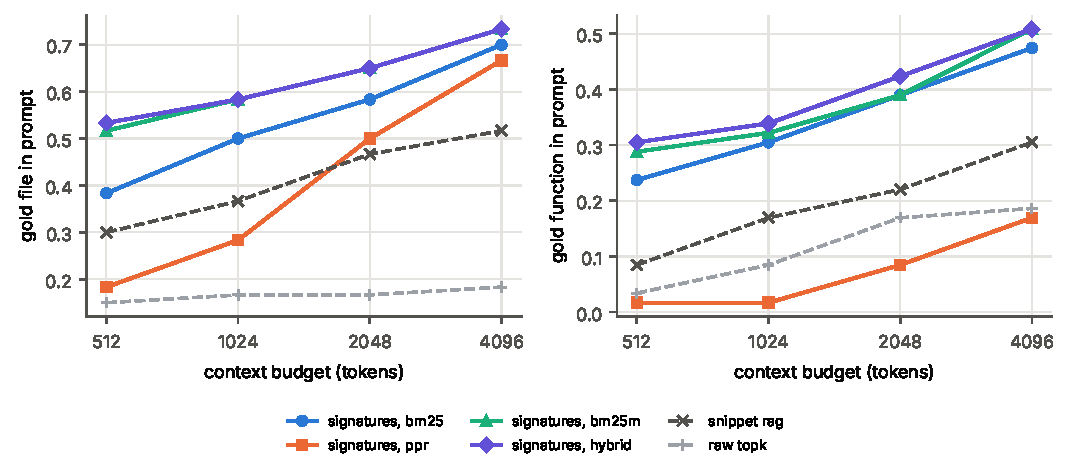
\includegraphics[width=\linewidth]{figs/fig_coverage.pdf}
\caption{Dev split ($n=60$, no LLM): fraction of prompts that contain the gold file (left) and the gold function definition (right), by context budget. Signature-map rankers are solid; text baselines dashed.}\label{fig:cov}\end{figure}

\subsection{Main comparison}
\begin{table}[t]\centering\small
\caption{Test split, $n=150$ (function accuracy on 119 instances), $B=2048$. Brackets are 95\% bootstrap intervals. Latency is end to end on a T4 including ingest.}\label{tab:main}
\begin{tabular}{@{}lccccccc@{}}\toprule
Method & File@1 & File@3 & Func@1 & ctx tok & prompt tok & p50 s & p95 s\\\midrule
issue only & 0.207 \ci{.147}{.273} & 0.253 & 0.109 \ci{.059}{.168} & 0 & 507 & 12.3 & 23.2\\
BM25 files (no LLM) & 0.267 \ci{.200}{.340} & 0.460 & -- & 0 & 0 & 4.7 & 15.9\\
raw top-$k$ & 0.280 \ci{.213}{.353} & 0.293 & 0.109 \ci{.059}{.168} & 2037 & 2548 & 13.4 & 25.1\\
snippet RAG & 0.380 \ci{.300}{.460} & 0.447 & 0.227 \ci{.160}{.303} & 2026 & 2558 & 13.8 & 26.2\\
\ours\ (edges + flow) & 0.487 \ci{.407}{.567} & 0.627 & 0.143 \ci{.084}{.210} & 2034 & 2592 & 17.6 & 28.2\\
\sig\ (signatures) & \textbf{0.527} \ci{.447}{.607} & \textbf{0.647} & \textbf{0.235} \ci{.160}{.311} & 2037 & 2595 & 17.0 & 29.8\\\bottomrule
\end{tabular}\end{table}

\begin{figure}[t]\centering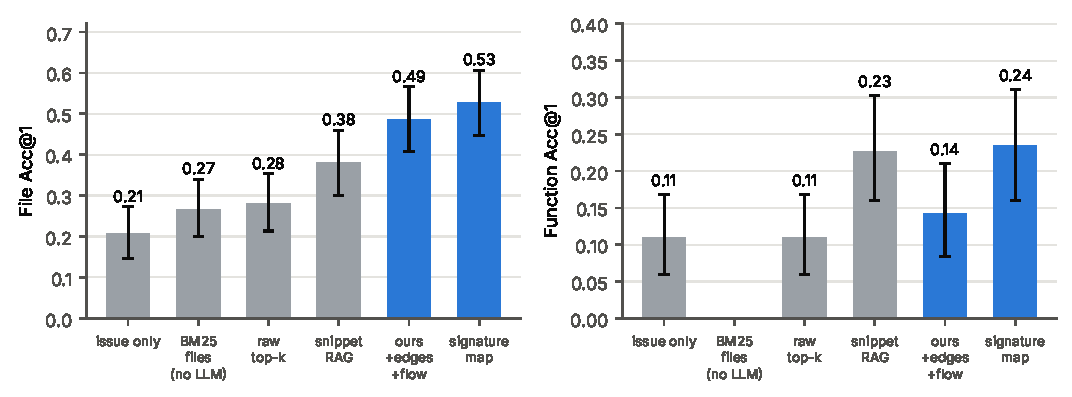
\includegraphics[width=.95\linewidth]{figs/fig_main.pdf}
\caption{Table~\ref{tab:main} as bars with 95\% intervals. Blue: graph methods.}\label{fig:main}\end{figure}

Table~\ref{tab:main} and Figure~\ref{fig:main} show the result we care about most: at the same 2k budget, a signature map locates the right file for 53\% of issues, snippet RAG for 38\% and raw files for 28\%. Against \sig, snippet RAG is 0.147 lower on file Acc@1 (95\% CI $-0.233$ to $-0.060$, $p_{\text{Holm}}=0.004$), raw top-$k$ 0.247 lower ($p_{\text{Holm}}<0.001$). The model with no context at all gets 0.207, so the 4B model is not guessing from the issue alone, but BM25 over files, with no LLM, already beats it on file@1 (0.267). Relative to BM25 file ranking the signature map is better by a factor of $0.527/0.267\approx1.97$ on File@1, which is the ``doubling'' quoted in the abstract.

Two things temper this. First, \ours{} is also well ahead of snippet RAG on files (+0.107, paired $p=0.023$, unadjusted, post hoc) but \emph{below} \sig{}: $-0.040$ on file Acc@1 (CI $-0.087$ to $+0.007$, $p_{\text{Holm}}=0.26$) and $-0.092$ on function Acc@1 (CI $-0.151$ to $-0.042$, $p_{\text{Holm}}=0.002$). Second, at function level snippet RAG is as good as the signature map (0.227 against 0.235, difference $-0.008$, $p=0.93$). A signature map shows names, not code; picking the function inside a file is a different problem from picking the file. Latency is 3--4 s higher for the graph methods at p50, mostly prefill on a longer prompt (about 3.0 s against 2.9 s median prefill) plus a longer answer (60 against 46 generated tokens).

\subsection{Ablations: edges, control flow, format, order}
\begin{table}[t]\centering\small
\caption{Ablations on the first 60 test instances (function accuracy on 48). Differences are against \sig\ in the top block and against \ours\ in the bottom block.}\label{tab:abl}
\begin{tabular}{@{}lccccc@{}}\toprule
Variant & File@1 & File@3 & Func@1 & prompt tok & $\Delta$file / $\Delta$func ($p_{\text{Holm}}$)\\\midrule
\sig\ & 0.500 & 0.650 & 0.188 & 2614 & reference\\
\; + edges & 0.467 & 0.667 & 0.125 & 2614 & $-.033$ (.78) / $-.062$ (.34)\\
\; + control flow & 0.533 & 0.683 & 0.208 & 2614 & $+.033$ (.88) / $+.021$ (.88)\\
\; \ours\ (both) & 0.417 & 0.617 & 0.042 & 2612 & $-.083$ (.08) / $-.146$ ($<$.001)\\
\; \sig\ with PPR ranker & 0.333 & 0.483 & 0.062 & 2612 & $-.167$ (.20) / $-.125$ (.29)\\\midrule
\ours\ & 0.417 & 0.617 & 0.042 & 2612 & reference\\
\; JSON rows instead of compact & 0.400 & 0.633 & 0.062 & 2597 & $-.017$ (1.0) / $+.021$ (1.0)\\
\; files alphabetical & 0.550 & 0.650 & 0.125 & 2605 & $+.133$ (.20) / $+.083$ (.60)\\
\; files shuffled & 0.467 & 0.650 & 0.146 & 2605 & $+.050$ (1.0) / $+.104$ (.053)\\
\; two-stage & 0.467 & 0.617 & 0.229 & 3803 & $+.050$ (.95) / $+.188$ (.003)\\\bottomrule
\end{tabular}\end{table}

Neither call edges nor control-flow counts helps on its own, and together they hurt function accuracy (Table~\ref{tab:abl}). The tokens they take are not free: with the budget fixed, every callee list pushes some other symbol out of the map, and the function-level gold is more often missing (dev coverage of the gold function at 2048 tokens drops from 0.42 for signatures to 0.29 for \ours). Whether the model also reads the extra columns badly we cannot say from this data. Control flow alone is nominally positive but far inside the noise.

Format and ordering effects are all unresolved at $n=60$. We note only that alphabetical and shuffled file order scored at least as well as relevance order, so we cannot claim that listing the most relevant file first helps this model. The old PPR-only ranker is clearly worse in point estimate (0.333 against 0.500), consistent with the dev coverage numbers, but the Holm-adjusted test does not reject.

The two-stage variant is the only change that moves function accuracy relative to \ours{}, but the fair comparison is \sig{}. Stage one shows the model only file names and symbol names (half the budget) and asks for candidate files; stage two re-renders the full map restricted to those files. With $M^{\mathrm{names}}_{B/2}$ the stage-one view and $M_B(\cdot\mid C)$ the map of Section~\ref{sec:method} restricted to a file set $C$,
\begin{equation}\label{eq:twostage}
C=\mathrm{LLM}\bigl(q,\,M^{\mathrm{names}}_{B/2}\bigr),\qquad (\hat F,\hat s)=\mathrm{LLM}\bigl(q,\,M_B(\cdot\mid C)\bigr).
\end{equation}
Function accuracy rises from 0.042 to 0.229 ($+0.188$, $p_{\text{Holm}}=0.003$) with file accuracy unchanged, at the cost of 1191 more prompt tokens and about 4.5 s more median latency (23.1 s against 18.6 s). Against \sig{} (0.188 on the same 48 instances) the difference is $+0.042$ on function accuracy (95\% CI $-0.062$ to $+0.146$, $p=0.54$) and $-0.033$ on file accuracy, so we cannot say that a second stage beats a single-stage signature map; \ours{} is an unusually low reference on this subset (0.042 here, 0.143 on all 150 test instances).

\subsection{Budget sweep}
\begin{figure}[t]\centering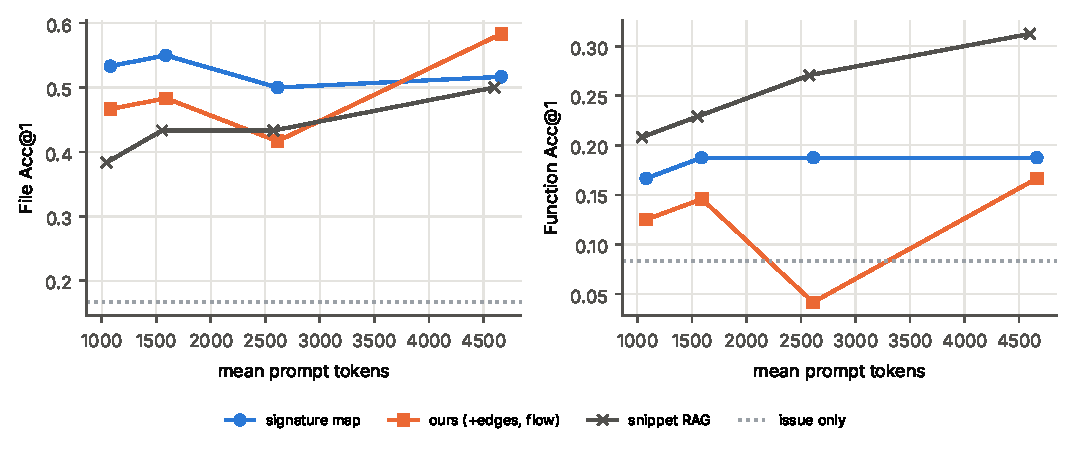
\includegraphics[width=\linewidth]{figs/fig_sweep.pdf}
\caption{Accuracy against mean prompt tokens on the first 60 test instances. Dotted: issue only (0.167 file, 0.083 function).}\label{fig:sweep}\end{figure}
Figure~\ref{fig:sweep} shows file accuracy for \sig\ is flat from about 1.1k to 4.7k prompt tokens (0.533, 0.550, 0.500, 0.517), so on this model more map does not give more localization. \ours\ is non-monotone (0.467, 0.483, 0.417, 0.583), which with $n=60$ and intervals of roughly $\pm0.12$ we read as noise rather than a trend. Snippet RAG improves steadily with budget, on files (0.383 to 0.500) and especially on functions (0.208 to 0.313), and has the highest function-level point estimate at every budget (the intervals overlap; at 4096 tokens the gap to \sig{} is $+0.125$, $p=0.094$). If the prompt is cheap and the goal is the function, bodies beat signatures; if the goal is the file and the prompt must be small, signatures win, and 512 tokens of map (about 1.1k prompt tokens) already gives most of the benefit.

\subsection{Where the failures are}
On the first 60 test instances the gold file is in the prompt for 78\% of issues with \ours\ (47/60) and 80\% with \sig\ (48/60). When it is absent the model never gets it right (0/13 and 0/12). When it is present, the model picks it first 53\% and 62\% of the time. Of the 35 failures with \ours\ (30 with \sig), 13 (12) are ranking misses; the remaining 22 (18) are cases where the right file was visible and the model chose a plausible neighbour: \texttt{django/db/models/query.py} for \texttt{django/db/models/sql/query.py}, \texttt{Dataset} for \texttt{DataArray} in xarray, a test file for the module under test. Per repository the picture is uneven (for example scikit-learn 0.79 and Django 0.64 for \sig, Flask 0.00 on a single instance); the repositories with few test instances are too small to say anything about.

\subsection{Memory and prefill on a T4}
\begin{figure}[t]\centering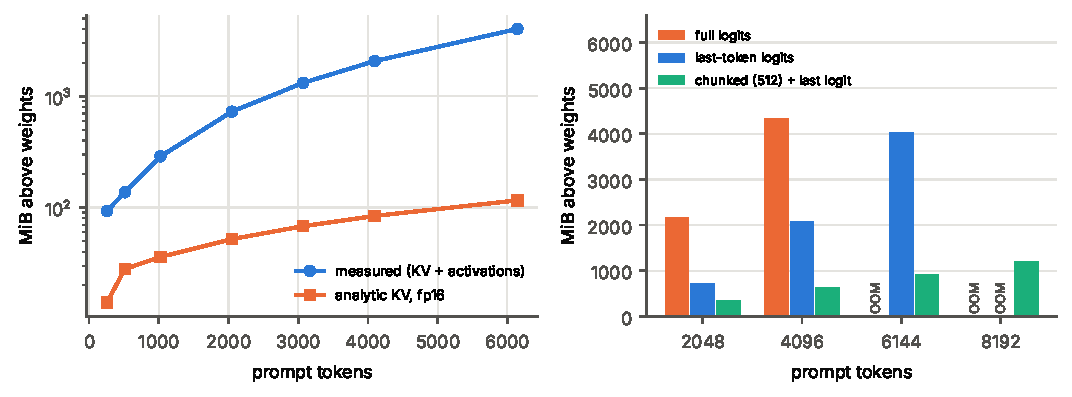
\includegraphics[width=\linewidth]{figs/fig_memory.pdf}
\caption{Left: memory above the weights during prefill, measured against the analytic fp16 KV cache (only the 24 layers that own a cache, sliding layers capped at 512 tokens). Right: peak extra memory by prefill strategy.}\label{fig:mem}\end{figure}
The checkpoint is not as small as ``4-bit'' suggests. Resident weights are 9081\,MiB. Of the 8802\,MiB of parameters, 5376\,MiB are per-layer embeddings and 1280\,MiB the token embedding, both left in bf16; only the 2146\,MiB of compute weights are quantized. The model has 42 layers (35 sliding-window with window 512, 7 full attention), 2 KV heads, head dimension 256 (512 in the full layers), and 18 layers share KV with earlier ones. Its analytic fp16 KV cache is therefore tiny: 14\,MiB at 256 tokens and 116\,MiB at 6144. With $n_{kv}=2$ heads and $\beta=2$ bytes per element, and, among the 24 layers that own a cache, $L_{\mathrm f}=4$ full-attention layers (head dimension $d_{\mathrm f}=512$) and $L_{\mathrm s}=20$ sliding layers ($d_{\mathrm s}=256$, window $w=512$), the cache for $n$ tokens is
\begin{equation}\label{eq:kv}
M_{\mathrm{KV}}(n)=2\,n_{kv}\,\beta\Bigl[L_{\mathrm f}\,d_{\mathrm f}\,n+L_{\mathrm s}\,d_{\mathrm s}\min(n,w)\Bigr]=
\begin{cases}56\ \mathrm{KiB}\cdot n, & n\le 512,\\[2pt] 16\ \mathrm{KiB}\cdot n+20\ \mathrm{MiB}, & n\ge 512,\end{cases}
\end{equation}
which reproduces both numbers above.

Measured memory above the weights is far larger (Figure~\ref{fig:mem}, left): 93\,MiB at 256 tokens, 727\,MiB at 2048, 4026\,MiB at 6144. Writing $\Delta M(n)$ for the measured memory above the weights, the KV share $M_{\mathrm{KV}}(n)/\Delta M(n)$ is $116/4026\approx3\%$ at 6144 tokens and at most about 20\% at any length. The rest is activations and logits, and the vocabulary of $V=262{,}144$ makes logits expensive: the logits for $m$ positions take $m\,V\beta$ bytes, which in fp16 is 2048\,MiB for $m=4096$ positions against 512\,KiB for the last position alone, the same order as the $4340-2069=2271$\,MiB saved below. Computing logits for every position at 4096 tokens costs 4340\,MiB above weights; asking only for the last position costs 2069\,MiB; prefilling in chunks of 512 with last-token logits costs 624\,MiB. At 6144 tokens, full logits run out of memory, and at 8192 only the chunked path runs (1191\,MiB, 15.4 s). These probes measure prefill memory on random token ids; we did not check answer quality at 8k tokens or the memory of decoding after a chunked prefill. Prefill time grows faster than linearly: 0.51 s at 512 tokens, 2.4 s at 2048, 9.0 s at 4096. Writing $T(n)\propto n^{\gamma}$, the local exponent is $\gamma=\ln(2.4/0.51)/\ln 4\approx1.1$ between 512 and 2048 tokens and $\gamma=\log_2(9.0/2.4)\approx1.9$ between 2048 and 4096.

Two conclusions follow for local deployment. A small prompt matters, but the thing it saves is mostly prefill time and activation memory, not KV cache; and chunked prefill with last-token logits is worth turning on before touching the context budget. We did not test KV-cache quantization or other quantization schemes.

\subsection{Compression ratio}
Over ten test instances, the full symbol graph of a repository (all symbols, signatures, edges, control flow) is on average $4.8\times$ smaller than its Python source, with source size estimated at 3.5 characters per token. For one instance let $T_{\mathrm{src}}$ be the source size in tokens (characters$/3.5$), $T_{\mathrm{graph}}$ the size of the full symbol graph and $T_{\mathrm{map}}\le B$ the size of the budgeted map. Then
\begin{equation}\label{eq:cr}
\rho_{\mathrm{total}}=\frac{T_{\mathrm{src}}}{T_{\mathrm{map}}}=\underbrace{\frac{T_{\mathrm{src}}}{T_{\mathrm{graph}}}}_{\rho_{\mathrm{AST}}}\cdot\underbrace{\frac{T_{\mathrm{graph}}}{T_{\mathrm{map}}}}_{\rho_{\mathrm{select}}}.
\end{equation} After ranking and budgeting to 2k tokens, the ratio is about $2300\times$ (range 500 to 4200). The first number is $\rho_{\mathrm{AST}}$, what AST compression buys on its own; the second is $\rho_{\mathrm{total}}$, which is mostly $\rho_{\mathrm{select}}$. We report both because the large one should not be credited to the parser.

\section{Using the index in a project}
The experiments use one configuration: the map is built before the call and prepended to the prompt. Two other uses follow from the results, and we implemented both in the released package.

\textbf{Prompt layer.} A function \texttt{RepoIndex.context(issue, budget)} returns the map; the caller prepends it to whatever prompt it already has. This works with any runtime, since it only needs a string, and is the setup measured above. The defaults are the best configuration found: signatures only, hybrid ranker.

\textbf{Tools.} The same index can be offered to the model as function-calling tools: \texttt{repo\_map}, \texttt{find\_symbol}, \texttt{read\_symbol}, \texttt{callers}, \texttt{callees}, \texttt{outline}; the package also wraps them as an MCP server. This follows from two findings. Edges did not help when serialized into the prompt, but they are useful to \emph{navigate}, so \texttt{callers} and \texttt{callees} make the graph available on demand without spending budget. And function-level accuracy only moved when the model was given a second, narrower view, which is what a \texttt{read\_symbol} call provides. We have unit-tested the tool layer and the agent loop against a scripted model; we have \textbf{not} yet measured it with Gemma~4, so this is a hypothesis, not a result. The experiment is described in the repository (\texttt{docs/integration.md}).

\section{Limitations}
\begin{itemize}\itemsep0pt
\item One model, one quantization, greedy decoding, one run. We have no variance across seeds or across Gemma sizes.
\item Localization only. We do not generate or test patches, so these numbers say nothing about resolve rate.
\item Intervals are wide. With 150 instances (60 for ablations) many comparisons are inconclusive; the ones we call results have Holm-adjusted $p<0.01$.
\item Python only. The parser is tree-sitter, so other languages need a grammar and the symbol rules, but we have not done it.
\item Name-based call resolution produces false edges for common names; the ``edges hurt'' result applies to this resolver and to how we serialize edges.
\item \sig\ is our own approximation of an Aider-style map. A comparison with the real tool, and with agentic search, is future work.
\item Dev and test splits share repositories, and we do not know whether SWE-bench Lite is in Gemma~4's training data.
\item Function accuracy is lenient (leaf-name match) and defined on a subset of instances.
\item End-to-end latency includes ingest with a warm parse cache and excludes symbol-scoring time (Section~3), so it is indicative rather than a cold-start figure.
\end{itemize}

\section{Conclusion}
For a 4B-effective local model with a 2k-token context budget, the useful part of an AST map is the ranked list of files and signatures; that alone doubles BM25 file ranking and beats code snippets and raw files on file localization. The additions we expected to help, call edges and control-flow counts in the prompt, did not. Function-level localization needs code bodies or a second stage, and snippet RAG is already as good as the map there. On a T4 the memory story is about logits and activations rather than KV cache. The next experiments are the tool-mode agent with Gemma~4, a hybrid that uses the map to pick files and snippet retrieval inside them, and more instances with several seeds.

\begin{thebibliography}{9}\small
\bibitem{swebench} C.~E. Jimenez et al. SWE-bench: Can language models resolve real-world GitHub issues? ICLR 2024. arXiv:2310.06770.
\bibitem{agentless} C.~S. Xia et al. Agentless: Demystifying LLM-based software engineering agents. 2024. arXiv:2407.01489.
\bibitem{aider} P. Gauthier. Building a better repository map with tree sitter. Aider documentation, \url{https://aider.chat/docs/repomap.html}.
\bibitem{repograph} S. Ouyang et al. RepoGraph: Enhancing AI software engineering with repository-level code graph. 2024. arXiv:2410.14684.
\bibitem{codexgraph} X. Liu et al. CodexGraph: Bridging large language models and code repositories via code graph databases. 2024. arXiv:2408.03910.
\bibitem{bm25} S. Robertson and H. Zaragoza. The probabilistic relevance framework: BM25 and beyond. Foundations and Trends in Information Retrieval 3(4), 2009.
\bibitem{pagerank} L. Page, S. Brin, R. Motwani, T. Winograd. The PageRank citation ranking: bringing order to the web. Stanford InfoLab technical report, 1999.
\bibitem{qlora} T. Dettmers et al. QLoRA: Efficient finetuning of quantized LLMs. NeurIPS 2023. arXiv:2305.14314.
\bibitem{ts} tree-sitter, \url{https://tree-sitter.github.io/}.
\bibitem{gemma} Gemma 4 E4B instruction-tuned, \texttt{google/gemma-4-E4B-it}, Hugging Face model card.
\end{thebibliography}
\end{document}
